    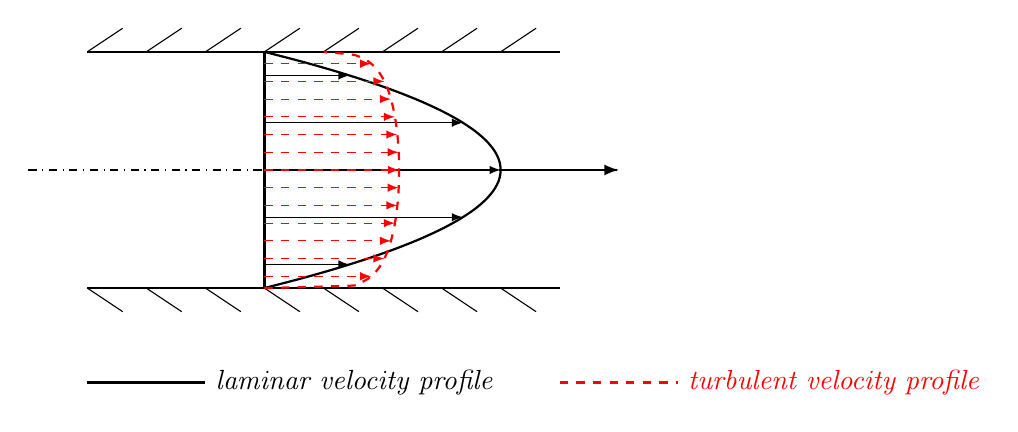
\begin{tikzpicture}[scale=1.5, >=latex]
        % --- SETTINGS ---
        \def\R{1.0}        % Pipe radius
        \def\L{4.0}        % Pipe length shown
        \def\UmaxLam{2.0}  % Max velocity laminar (Higher peak)
        \def\UmaxTurb{1.14} % Max velocity turbulent: same flow rate as laminar (mean velocity 1.0 in both cases)
        
        % --- PIPE WALLS ---
        \draw[thick] (0, \R) -- (\L, \R);
        \draw[thick] (0, -\R) -- (\L, -\R);
        
        % Wall Hatching
        \foreach \x in {0, 0.5, ..., 3.5} {
            \draw (\x, \R) -- (\x+0.3, \R+0.2);
            \draw (\x, -\R) -- (\x+0.3, -\R-0.2);
        }
        
        % Centerline
        \draw[dashdotted] (-0.5, 0) -- (\L+0.5, 0);
        \draw[->, thick] (\L-0.5, 0) -- (\L+0.5, 0); 

        % =========================================
        % LAMINAR PROFILE (Parabolic - Solid Black)
        % =========================================
        % u(y) = UmaxLam * (1 - (y/R)^2)
        \draw[thick] (1.5, \R) -- (1.5, -\R); % Vertical start line
        \draw[thick, smooth, domain=-\R:\R] plot ({1.5 + \UmaxLam*(1 - (\x/\R)^2)}, \x);
        
        % Arrows for Laminar
        \foreach \y in {-0.8, -0.4, 0, 0.4, 0.8} {
            \draw[->, thin] (1.5, \y) -- ({1.5 + \UmaxLam*(1 - (\y/\R)^2)}, \y);
        }

        % =========================================
        % TURBULENT PROFILE (Modified Power Law - Dashed Red)
        % =========================================
        % Using (1 - (r/R)^2)^0.14 instead of (1 - r/R)^0.14
        % This forces the derivative to be 0 at r=0, creating a smooth flat peak.
        \draw[thick, red, dashed, smooth, domain=-\R:\R, samples=100] plot ({1.5 + \UmaxTurb*pow(1 - (\x/\R)^2, 0.14)}, \x);
        
        % Arrows for Turbulent (Dense arrows to show the profile)
        \foreach \y in {-0.9, -0.75, -0.6, -0.45, -0.3, -0.15, 0, 0.15, 0.3, 0.45, 0.6, 0.75, 0.9} {
            \draw[->, red, dashed, thin] (1.5, \y) -- ({1.5 + \UmaxTurb*pow(1 - (\y/\R)^2, 0.14)}, \y);
        }

        % --- LEGEND ---
        \begin{scope}[shift={(0, -1.8)}]
            \draw[thick] (0, 0) -- (1, 0) node[right] {\textit{laminar velocity profile}};
            \draw[thick, red, dashed] (4, 0) -- (5, 0) node[right, align=left] {\textit{turbulent velocity profile}};
        \end{scope}

    \end{tikzpicture}
